\section{Zielsetzung}
\label{sec:Zielsetzung}

Ziel des Versuches ist es, die Abhängigkeit der Intensität des, an einem Silizium-Spiegel reflektierten, Lichtes vom Eintrittswinkel und der Polarisation zu bestimmen und somit den Brechungsindex von Silizium zu berechnen.. 

\section{Theorie}
\label{sec:Theorie}

Beim Durchqueren von Grenzflächen zweier Medien mit verschiedenen Brechungsindizes, wird das sich ausbreitende Licht in den meisten Fällen sowohl reflektiert, als
auch gebrochen. Um zu bestimmen, welchen Anteil der ursprünglichen Intensität des einfallenden Lichtes das reflektierte und das gebrochene Licht haben, wird
zunächst ein allgemeiner Ausdruck für die Strahlungsleistung von Lichtwellen benötigt.
\newline
Aus den Maxwell Gleichungen und der Elektrizitätslehre folgt der Audruck 
\begin{equation}
    \vec{S} = \vec{E} \times \vec{H},
\end{equation}
wobei $\vec{E}$ die elektrische und $\vec{H}$ die magnetische Feldstärke einer elektromagnetischen Welle beschreiben. $\vec{S}$ wird als Poynting-Vektor bezeichnet
und hat die Dimension $\frac{\text{Leistung}}{\text{Fläche}}$. Er beschreibt den Transport von Energie, da er in die Ausbreitungsrichtung der elektromagnetischen
Welle zeigt und sein Betrag dem der Energie der Strahlung entspricht.

\begin{figure}[H]
	\centering
	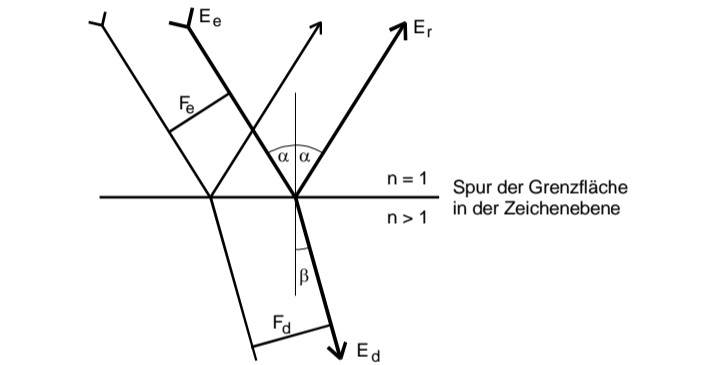
\includegraphics[width=0.6\linewidth]{data/v407Brechung.jpg}
	\caption{Reflektion eines Lichtstrahls an einer Grenzfläche.\cite{Anleitung407}}
	\label{fig:brechung}
\end{figure}

\noindent
Trifft eine elektromagnetische Welle nun auf eine Grenzfläche zwischen zwei Medien, teilt sich ihre Strahlungsleistung auf den reflektierten und gebrochene Teil auf.
Da in diesem Versuch ausschließlich nicht absorbierende Medien betrachtet werden, gilt mit der Energieerhaltung
\begin{equation}
    S_\text{e} \cos(\alpha) = S_\text{r} \cos(\alpha) + S_\text{d} \cos(\alpha).
\end{equation}
Hierbei bezeichnet $S_\text{e}$ den Betrag des Poynting-Vektors der einfallenden und $S_\text{r}$ und $S_\text{d}$ analog den der reflektierten und gebrochenen Strahlung.
$\alpha$ ist in diesem Fall der Winkel, in dem die einfallende Strahlung auf die Grenzfläche trifft und $\beta$ der, in dem sich die gebrochene Strahlung von der Grenzfläche
entfernt.
\newline
Aus diesen beiden Winkeln lässt sich mit Hilfe des Snelliusschen Brechungsgesetzes ein Audruck für den Brechungsindex $n$ finden
\begin{equation}
    n = \frac{\sin(\alpha)}{\sin(\beta)}.
\end{equation}
Dieser Brechungsindex beschreibt außerdem das Verhältniss der Geschwindigkeit von Licht in beiden Medien. Es gilt
\begin{equation}
    n = \frac{c}{v}.
\end{equation}
\newline\newline
Da das Verhältnis zwischen reflektiertem und gebrochenem Anteil der Strahlung stark vom Polarisationszustand dieser abhängig ist, müssen im Folgenden senkrecht und
parallel zur Grenzfläche polarisierte Stahlungsanteile seperat betrachtet werden.
Für senkrecht polarisierte Strahlung gilt durch vorherige Überlegungen
\begin{equation}
    \vec{E_{\text{r}\perp}}(\alpha) = \vec{E_{\text{e}\perp}} \frac{(\sqrt{n^2 - \sin^2(\alpha)} - \cos(\alpha))^2}{n^2 - 1}.
    \label{eqn:fresnelsenk}
\end{equation}
Für parallel polarisierte Strahlung gilt analog
\begin{equation}
    \vec{E_{\text{r}\parallel}}(\alpha) = \vec{E_{\text{e}\parallel}} \frac{n^2 \cos(\alpha) + \sqrt{n^2} - \sin^2(\alpha)}{n^2 \cos(\alpha) - \sqrt{n^2} - \sin^2(\alpha)},
    \label{eqn:fresnelpara}
\end{equation}
wobei in beiden Relationen $n$ der Brechungsindex und $\alpha$ der Winkel in dem die Strahlung auf die Grenzfläche trifft ist. $\vec{E_{\text{r}}}$ und
$\vec{E_{\text{e}}}$ geben jeweils die Amplituden der elektrischen Felder für den reflektierten und einfallenden Teil der Strahlung an.
\newline\newline
Der Ausdruck für $\vec{E_{\text{r}\parallel}}(\alpha)$ lässt sich auch schreiben als
\begin{equation}
    \vec{E_{\text{r}\parallel}}(\alpha) = \vec{E_{\text{e}\parallel}} \frac{\tan(\alpha - \beta)}{\tan(\alpha + \beta)}.
\end{equation}
Daraus folgt, dass $\vec{E_{\text{r}\parallel}}(\alpha)$ Null werden kann, insofern die Voraussetzung $\alpha + \beta = 90°$ erfüllt ist. Es verschwindet somit für einen bestimmten
Winkel von $\alpha$ der gesamte reflektierte Anteil und die gesamte Strahlung tritt in das brechende Medium ein. Dieser bestimmte Winkel wird Brewster Winkel gennant und durch die folgende Relation ausgedrückt
\begin{align}
    \arctan(n) = \alpha_{\text B}.
\end{align}